%File: formatting-instruction.tex
\documentclass[letterpaper]{article}
\usepackage{url,graphicx,xcolor}
\usepackage{times}
\usepackage{helvet}
\usepackage{courier}
\usepackage{hyperref}
\usepackage[guidelines]{faikrmod3}
% \usepackage[]{faikrmod3}
% \usepackage[]{faikrmod3} % without guidelines
\frenchspacing
\setlength{\pdfpagewidth}{8.5in}
\setlength{\pdfpageheight}{11in}



% THE \pdfinfo /Title AND /Author ARE NOT NECESSARY, THEY ARE METADATA FOR THE FINAL PDF FILE
\pdfinfo{
/Title (Insert Your Title Here)
/Author (Put All Your Authors Here, Separated by Commas)}
\setcounter{secnumdepth}{0}  
 \begin{document}
% The file aaai.sty is the style file for AAAI Press 
% proceedings, working notes, and technical reports.
%
\title{Interpretable Diabetes Risk Analysis Using Bayesian Networks}
\author{Sara Tajernia, Mohammad Choupan, Mohammad Amin Mirzakuchaki\\
Master's Degree in Artificial Intelligence, University of Bologna\\
\{ sara.tajernia, mohammad.choupan, mohamma.mirzakuchaki \}@studio.unibo.it
}
\maketitle

\begin{abstract}
\begin{quote}

\explanation{
This project explores the use of Bayesian Networks for modeling diabetes risk using the Pima Indians Diabetes dataset. Different strategies for handling missing values encoded as zeros are compared, and a drop-based approach is selected based on correlation structure preservation. Continuous variables are discretized to support Bayesian Network modeling. Several network structures are analyzed, including a naïve Bayes–like model, a manually defined grouped-feature model, and data-driven structures learned using Tree Search and Hill Climbing algorithms. These models are evaluated through probabilistic inference to analyze how diabetes risk varies under controlled changes of key factors. Additionally, Hill Climbing–based Bayesian Networks are assessed in a classification setting to evaluate predictive performance.
}

\end{quote}
\end{abstract}


\section{Introduction}
\subsection{Domain}

\explanation{
Diabetes mellitus is a chronic metabolic disease characterized by elevated blood glucose levels, which can lead to severe health complications if not properly managed. The risk of developing diabetes is influenced by multiple factors, including demographic characteristics, physiological measurements, and genetic predisposition. Understanding how these factors interact is important for both early diagnosis and risk assessment. \\
In this project, diabetes risk is studied using the Pima Indians Diabetes dataset \cite{uci_diabetes}, which contains medical records of female patients, including variables such as age, body mass index (BMI), blood pressure, glucose concentration, insulin level, number of pregnancies, and a diabetes pedigree function representing genetic risk. The dataset provides a suitable setting for exploring how combinations of risk factors contribute to the likelihood of diabetes.
}

\subsection{Aim}
\explanation{
We study the effect of key variables such as age, body mass index, glucose level, and genetic predisposition, and compare different Bayesian Network structures, including manually defined models and data-driven structure learning approaches. Through probabilistic inference, we assess the ability of these models to capture meaningful relationships between risk factors and to provide interpretable insights into diabetes risk. 
}

\subsection{Method}
\explanation{
The analysis is conducted using the Pima Indians Diabetes dataset. Several preprocessing strategies are explored to handle missing values encoded as zeros, including row dropping and imputation-based approaches. Based on correlation analysis and data consistency considerations, a drop-based strategy is selected for the final analysis. Continuous variables are then discretized into categorical bins to support Bayesian Network modeling. \\
Bayesian Networks are implemented using the pgmpy \cite{pgmpy} library to define network structures, estimate parameters, and perform probabilistic inference. Multiple structures are considered, including a naïve Bayes–like baseline model, a manually defined grouped-feature model, and data-driven structures learned using Tree Search and Hill Climbing algorithms with different scoring functions. For each model, conditional probability tables are estimated using maximum likelihood estimation. \\
Model evaluation is performed through probabilistic inference by fixing subsets of variables and systematically varying others, allowing the posterior probability of diabetes to be analyzed under controlled scenarios. In addition, Bayesian Networks learned via Hill Climbing are evaluated in a classification setting to assess their predictive performance alongside the inference-based analysis.
}


\subsection{Results}
\explanation{
The experiments show that Bayesian Network behavior is strongly affected by preprocessing and structure choices. Simple or manually defined structures often produced unstable or uninformative posterior probabilities, whereas models learned from data yielded more coherent inference results. \\
In particular, combinations of appropriate imputation and discretization methods led to posterior diabetes risk estimates that were more consistent and interpretable across different evidence configurations.
}


\section{Model}
\begin{figure}
    \centering
    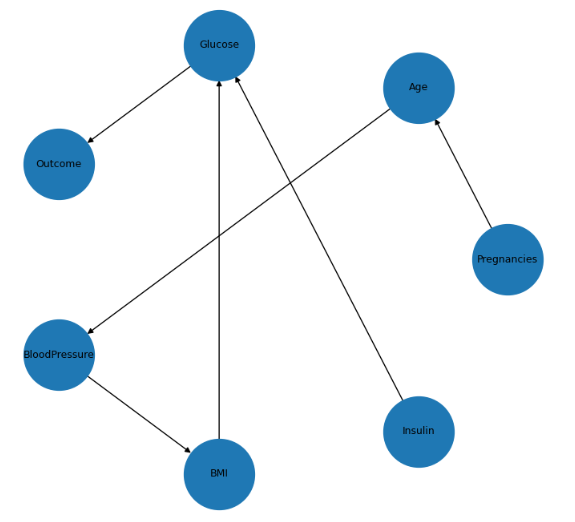
\includegraphics[width=0.8\linewidth]{hc_aic.png}
    \caption{Bayesian Network structure learned using Hill Climbing with AIC score, selected as one of the best-performing models for probabilistic inference and classification.}
    \label{fig:network}
\end{figure}
% }

\explanation{
Figure~\ref{fig:network} illustrates a representative Bayesian Network used in this project, corresponding to a structure learned using Hill Climbing with the AIC scoring function. The network includes nodes representing clinical and demographic variables such as glucose concentration, body mass index, age, blood pressure, insulin level, number of pregnancies, and a diabetes pedigree function, together with a binary node representing diabetes outcome. \\
Continuous variables are discretized into a finite number of categorical states to enable parameter learning and probabilistic inference. Conditional probability tables are estimated from the discretized dataset using maximum likelihood estimation. While this figure shows a single learned structure for clarity, additional network structures—including a naïve Bayes–like baseline, a manually defined model, and alternative data-driven structures—are explored and compared in the subsequent analysis to assess the impact of structural assumptions on inference behavior.
}


\section{Analysis}

\subsection{Experimental setup}
\explanation{
The analysis is based on probabilistic inference queries aimed at evaluating how changes in selected clinical variables affect the posterior probability of diabetes. For each Bayesian Network model, we compute the posterior probability of the Outcome node under controlled evidence configurations involving variables such as glucose concentration, age, body mass index, number of pregnancies, and genetic risk. \\
Experiments are conducted by fixing one or more variables to representative categorical values while systematically varying another variable across its discretized range. This enables the analysis of diabetes risk trends under controlled conditions, such as increasing age at high glucose levels or varying body mass index for specific age groups. The same set of queries is applied across different network structures to allow direct comparison. \\
Results are evaluated qualitatively by examining posterior probability trends, with attention to sensitivity to evidence, monotonic behavior, and clinical plausibility. The focus is on interpretability and the influence of structural assumptions rather than on predictive accuracy.
}


\subsection{Results}
\begin{itemize}
    \item \textbf{Inference and Query Results:}  
    Inference results reveal substantial sensitivity differences across Bayesian Network structures. Simple models, such as Na\"ive Bayes--like and tree-based networks, show minimal changes in posterior diabetes probability under varying evidence (typically below 2\%). In contrast, models with richer dependency structures respond more strongly to changes in risk factors. The grouped model captures clear increases in inferred diabetes risk for fixed high glucose levels (approximately +25 percentage points), elderly individuals as glucose levels rise (exceeding 70 percentage points), and high genetic risk combined with increasing numbers of pregnancies (around +30 percentage points), highlighting the impact of structural assumptions on inferred risk.

    \item \textbf{Classifier Performance:}  
    The selected Hill Climbing model using the AIC score achieved a mean classification accuracy of 75.1\% ($\pm$4.1\%) under 10-fold cross-validation, supporting its use as a representative structure for both probabilistic inference and prediction.
\end{itemize}
% \explanation{
% Inference results show substantial differences in sensitivity across Bayesian Network structures. Simple models, such as the naïve Bayes–like and tree-based networks, exhibit little to no change in posterior diabetes probability under varying evidence (typically below 2\%). In contrast, models with richer dependency structures respond more strongly to changes in risk factors. \\
% When age increases under fixed high glucose levels, the grouped model shows a clear rise in inferred diabetes risk (approximately +25 percentage points), while simpler models remain nearly flat. Similarly, Hill Climbing–learned models display sharp increases in diabetes probability for elderly individuals as glucose levels rise, with changes exceeding 70 percentage points. Finally, when genetic risk is high, the grouped model captures a notable increase in diabetes probability as the number of pregnancies increases (around +30 percentage points). These findings highlight the impact of structural assumptions on the magnitude and plausibility of inferred risk. \\
% The selected Hill Climbing (AIC) model also achieved a mean accuracy of 75.1\% (±4.1\%) under 10-fold cross-validation, supporting its use as a representative structure.
% }



\section{Conclusion}
\explanation{
This project explored Bayesian Networks for modeling diabetes risk and showed that inference results are highly sensitive to preprocessing choices and network structure. Simple models often produced nearly flat risk estimates, while data-driven structures learned via hill climbing captured more meaningful variations in diabetes probability under changing evidence. Overall, the study highlights both the interpretability of Bayesian Networks and their limitations when applied to small, discretized datasets.
}

\section{Links to external resources}
\explanation{
\raggedright
GitHub repository: \href{https://github.com/sara-tajernia/Diabetes-Analysis-with-Bayesian-Network/}{github.com/sara-tajernia/Diabetes-Analysis-with-Bayesian-Network}
}

\bigskip

\bibliographystyle{aaai}
\bibliography{faikrmod3.bib}
% \cite{uci_diabetes}
% \cite{pgmpy}
% \cite{scikit_learn}

% \attention{NOTICE: THIS REPORT'S LENGTH MUST NOT EXCEED \textbf{TWO PAGES} PLUS REFERENCES. THIS MAY MEAN THAT YOU WILL HAVE TO LEAVE OUT OF THE REPORT PART OF THE WORK YOU HAVE DONE OR OBSERVATIONS YOU HAVE. THIS IS NORMAL: THE REPORT SHOULD EMPHASIZE WHAT IS MOST SIGNIFICANT, NOTEWORTHY, AND REFER TO THE NOTEBOOK FOR ANYTHING ELSE. FOR ANY OTHER ASPECT OF YOUR WORK THAT YOU WOULD LIKE TO EMPHASIZE BUT CANNOT EXPLAIN HERE FOR LACK OF SPACE, FEEL FREE TO ADD COMMENTS IN THE NOTEBOOK.}



\end{document}